\documentclass[10pt]{article}

\usepackage{amsmath}
\usepackage{fullpage}
\usepackage{array}
\usepackage{graphicx}
\usepackage{gensymb}
\usepackage{booktabs}
\usepackage{gensymb}
\usepackage{graphicx}

\graphicspath{ {../Images/} }

\date{2017-10-11}
\pagestyle{empty}
\setlength{\parindent}{0pt}

\begin{document}
\begin{center}
\begin{Large}\textbf{Chapter: Kinetic Energy and Work}\end{Large} \\
\smallskip
%\begin{large} Acceleration \end{large}
\end{center}
%%%%%%%
Objectives: Apply the relationship between a particle's kinetic energy, mass and speed, qualitative understanding of work-energy theorem, identify work as scalar product. 
\section{Energy}
Vauge definition: Energy is a scalar quantity associated with the state or condition of the system. 
Athletes on tracks feel \emph{energized}. That is essentially due to the particular hormone known as adrenaline.  It enhances the metabolism rate and prepares the muscles for exertion.  I feel energized while doing research and teaching!


\subsection{Kinetic Energy}
\textbf{Kinetic Energy} $K$ is associated with the \emph{state of motion} of an object.  The faster the object moves, the greater its kinetic energy is.

Consider a  point particle with the mass $m$ moving with the \emph{speed} $v$\footnote{Relativistically speaking $v$ should be very small than the speed of light which is $3\times 10^8$ m/s.  It is true since the maximum speeds we deal with are of the order of 100 m/s.}.  Then the kinetic energy is given by
\begin{equation}
  K = \frac{1}{2}mv^2
\end{equation}
The units of kinetic energy can be found as follows.  In SI units, mass $m$ is measured in kg and speed $v$ is in m/s.  Thus the SI units for kinetic energy is kg.$\text{m}^2/\text{s}^2$.  This is exactly equal to 1 joule.

\subsection{Work}
In the previous section we considered a particle with mass $m$ moving with speed $v$.  Now \emph{someone} (or something) applied some force on the particle to accelerate it upto that speed.  That means that some \emph{work} was done on the particle. 

Roughly, work $W$ is the energy transferred to or from an object via a force acting on the object.  Energy transferred to the object is the positive work, and from the object, negative work.  [Explain the term transfer!]

Mathematically, work is a scalar product of vector force $\vec{F}$ and vector displacement $\vec{d}$.  
\begin{equation}
\begin{split}
  W &= \vec{F}.\vec{d}\\
    &= Fd\cos\theta
\end{split}
\end{equation}
\begin{figure}[h]
\label{Scalar product}
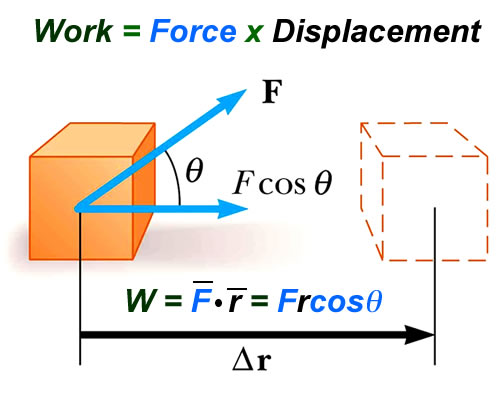
\includegraphics[scale=.5]{workd}
\centering
\end{figure}
\newpage
\textbf{Cautions}
\begin{enumerate}
\item The force $\vec{F}$ should be constant during the motion of the object.\footnote{For variable forces we use calculus by demanding that $\vec{F}$ is constant for an \emph{infinitesimal} motion!}
\item Objects should be point particles.
\end{enumerate}

\subsection{Work-Kinetic energy theorem}
The theorem states that the work done by \emph{all} the forces on an object is equal to the change in the kinetic energy of the object.
\begin{equation}
  \Delta K = K_f-K_i = W
\end{equation}

\subsection{Work done by gravity}
\begin{figure}[h]
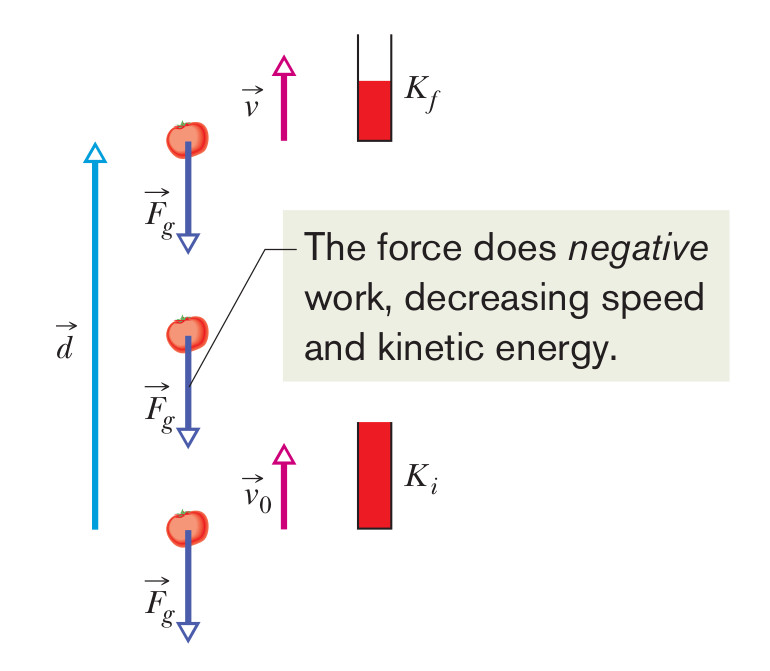
\includegraphics[scale=.9]{gravwork}
\centering
\caption{Tomato thrown upwards}
\label{workdgrav}
\end{figure}
Consider a tomato of mass $m$ thrown upwards with the initial speed $v_0$.  Thus the initial kinetic energy of the tomato is $\frac{1}{2}mv_0^2$.  Now there is only one force acting on the tomato in the downward direction.  This is the force of gravity as shown in the figure \ref{workdgrav}.  Now our daily experience suggests that the tomato should slow down as it gains height.  This is essentially because gravity is doing negative work on the tomato.  The work done is
\begin{equation}
  \begin{split}
    W_g&=F_gd\cos\theta\\
       &= mgd\cos\theta\\
       &= mgd\cos 180\\
       &= -mgd
  \end{split}
\end{equation}

\subsection{Work done in lifting and lowering an object}
Consider lifting up a particle vertically up with the force $\vec{F}$.  Let the work done by this force be $W_a$.  Now we can convince ourselves that work done by gravity, during the lift, should be negative.  Let us further assume that we lift the particle slowly enough to not to change its speed.  Thus the change in kinetic energy $\Delta K=0$.

Now we apply the work energy theorem
\begin{equation}
\begin{split}
\Delta K &= K_f-K_i\\
&= W_a+W_g\\
&=0
\end{split}
\end{equation}
This implies, $W_a=-W_g$.

\section{Answer the followig question}
\begin{enumerate}
\item The figure below shows an overhead view of the three horizontal forces acting on a cargo canister that was initially stationary but now moves across a frictionless floor.  The force magnitudes are $F_1=3N$, $F_2=4N$, and $F_3=10N$.  The indicated angles are $\theta_2=50^\circ$ and $\theta_3=35^\circ$.  What is the net work done by all the forces during the first 4m of the displacement? What is the final speed of the box if it started from rest (assume the mass $m=5$kg)?
\begin{figure}[h]
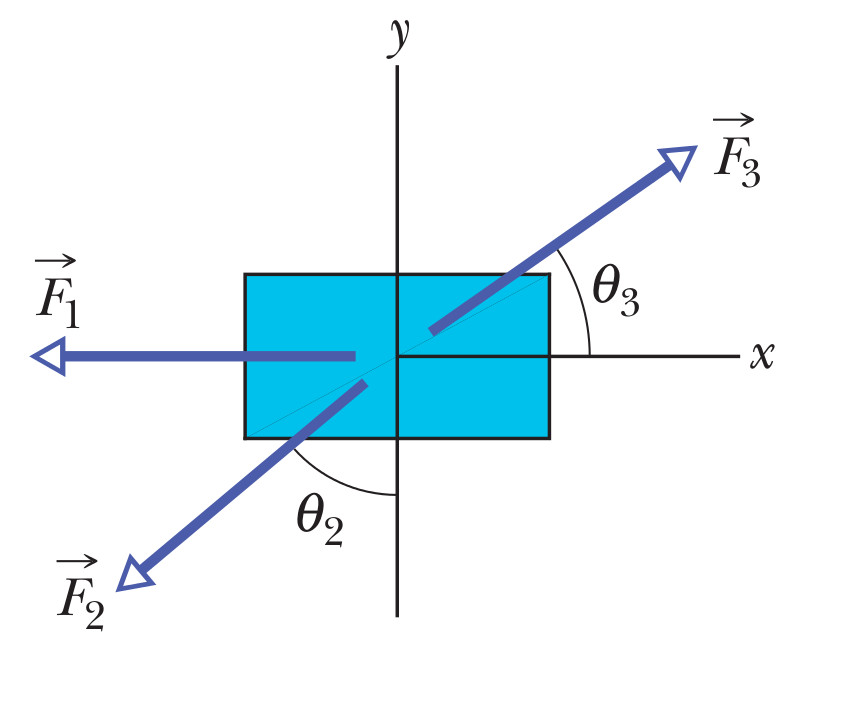
\includegraphics[scale=1.2]{workonbox}
\centering
\end{figure}
\end{enumerate}
\end{document}
